\subsection{Decision Tree from Scratch}
We implemented a deterministic, binary, axis-aligned decision tree in NumPy for both tasks. Classification uses either Gini impurity $1-\sum_k p_k^2$ or base-2 entropy $-\sum_k p_k\log_2 p_k$; regression uses within-node mean squared error, $N^{-1}\sum_i(y_i-\bar y)^2$. Each feature is sorted and candidate thresholds are midpoints between adjacent distinct values. Prefix class counts or prefix sums of targets and squared targets evaluate all candidate impurity reductions in linear time after sorting. A split must leave at least \texttt{min\_samples\_leaf} rows on each side. Growth also obeys \texttt{max\_depth}, \texttt{min\_samples\_split}, and \texttt{min\_impurity\_decrease}; the latter uses node-size-weighted gain, matching scikit-learn's convention. Classification leaves predict the majority class and expose empirical class frequencies through \texttt{predict\_proba}; regression leaves predict the mean. Feature importance sums the training-sample-weighted impurity decrease per feature and is normalized to one. With $m$ rows and $d$ features in a node, split search takes $O(dm\log m)$ time for the sorts and $O(mK)$ temporary memory for $K$ classes. An individual prediction follows one root-to-leaf path.

\subsection{Tree Experiments and Matched Baseline}
The tree-only experiment uses version 1 of the Kaggle \emph{Binaaz sale project} dataset\footnote{\url{https://www.kaggle.com/datasets/sehriyarmemmedli/binaaz-sale-project}}. It keeps the latest scrape of each listing URL, removes target-derived values and identifiers from the feature set, converts area, rooms, floor, land area (sot to $\mathrm{m}^2$), and currency, and applies fixed plausibility bounds (5{,}000--20{,}000{,}000 AZN for price; 10--2{,}000 $\mathrm{m}^2$ for observed floor area). All 100{,}775 rows have AZN currency; 62{,}703 rows remain after deduplication and filtering. Stratification uses predeclared AZN price bands, yielding 43{,}891 training, 9{,}406 validation, and 9{,}406 test rows. The tier threshold is the training median, 212{,}000 AZN. Numeric medians, the top 25 locations, and one-hot columns are learned from training rows only. There are 58 model features. Because the Python/NumPy tree is a teaching implementation, both tree models and their sklearn counterparts fit the same seeded 5{,}000-row sample of the training split; validation and test metrics use their full respective splits.

We model $\log(\text{price})$ for Task A and exponentiate predictions for AZN metrics. Maximum depth was swept from 1 to 20 with five samples per leaf; the leaf minimum was then checked at 1, 5, and 20 at the selected depth. Task B compared Gini and entropy at every depth. Selection used validation RMSE for Task A and validation F1 (AUC as tie-breaker) for Task B. The selected regression tree has depth 8 and minimum leaf size 5; the classification tree uses Gini, depth 9, and minimum leaf size 1. Other stopping parameters stayed at \texttt{min\_samples\_split=2} and \texttt{min\_impurity\_decrease=0}. The final test split was read only after those choices. Matched scikit-learn trees\footnote{\url{https://scikit-learn.org/stable/modules/tree.html}} use the same fitting rows and structural parameters, with \texttt{random\_state=42}.

\begin{table}[t]
\centering
\caption{Tree test metrics on 9{,}406 held-out listings. Times are single-run seconds on the same machine.}
\label{tab:tree_results}
\resizebox{\columnwidth}{!}{%
\begin{tabular}{@{}llrrrr@{}}
\toprule
Task & Model & RMSE (AZN) & MAE (AZN) & $R^2$ & fit/predict (s) \\
\midrule
A & Ours & 391{,}531 & 99{,}840 & 0.45256 & $\sim$0.13/0.011 \\
A & sklearn & 391{,}531 & 99{,}840 & 0.45256 & $\sim$0.016/0.002 \\
\midrule
Task & Model & Precision & Recall & F1/AUC & fit/predict (s) \\
\midrule
B & Ours & 0.8905 & 0.9001 & 0.8952/0.9251 & $\sim$0.26/0.010 \\
B & sklearn & 0.8910 & 0.9003 & 0.8956/0.9246 & $\sim$0.014/0.001 \\
\bottomrule
\end{tabular}
}
\end{table}

Task B's own-tree precision and recall are 0.8905 and 0.9001, with confusion matrix $\left[\begin{smallmatrix}4170&522\\471&4243\end{smallmatrix}\right]$ in $[\mathrm{TN},\mathrm{FP};\mathrm{FN},\mathrm{TP}]$ order. Task A's sklearn RMSE matches ours to the displayed precision, while Task B F1 and AUC differ slightly because of implementation details and tie-breaking. The NumPy implementation fits more slowly than the compiled sklearn tree. These holdout scores are single-split estimates; cross-validation uncertainty belongs in the team's combined benchmark table.

\begin{figure}[t]
\centering
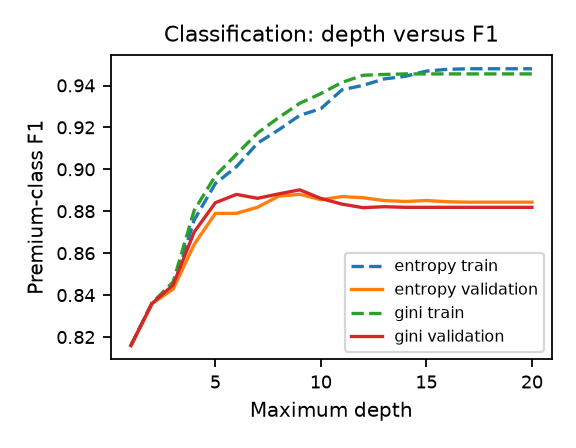
\includegraphics[width=\linewidth]{figures/tree_classification_depth.png}
\caption{Training and validation F1 for Gini and entropy as maximum depth increases (minimum leaf size 5). The widening train-validation gap at greater depth indicates overfitting.}
\label{fig:tree_depth}
\end{figure}

\subsection{Tree Error Analysis}
For regression, floor area accounts for 0.611 of normalized impurity-decrease importance; house/villa category (0.112), longitude (0.090), and land area (0.058) follow. In classification, floor area accounts for 0.563 and longitude for 0.149. Impurity-based importance favors continuous or high-cardinality features, so these are descriptive model diagnostics, not causal effects. The overall test MAE is 99{,}840 AZN, rising to 547{,}009 AZN among 939 listings above the training price 90th percentile and to 663{,}872 AZN for 275 land plots. The overall classification error rate is 10.6\%, but it reaches 35.9\% for 1{,}053 test prices within 10\% of the training tier threshold and 19.6\% for land plots. These groups differ in price range and sample size, so the contrasts identify where to inspect failures rather than prove why they occur.

\begin{figure}[t]
\centering
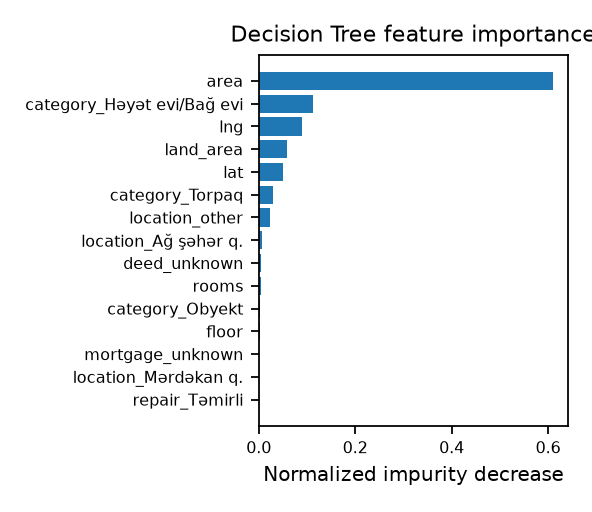
\includegraphics[width=\linewidth]{figures/tree_regression_importance.png}
\caption{Top regression-tree features by normalized impurity decrease.}
\label{fig:tree_importance}
\end{figure}

\paragraph{AI assistance disclosure.} OpenAI Codex assisted with implementing, testing, benchmarking, and drafting this Decision Tree section. Ilaha Gadirli is responsible for reviewing it before final submission.
